\documentclass[border=4pt]{standalone}
\usepackage{amsmath,amssymb,pgfplots}\pgfplotsset{compat=1.18}
\definecolor{figB}{RGB}{31,90,166}\definecolor{figR}{RGB}{176,48,48}\definecolor{figG}{RGB}{46,125,50}\definecolor{figO}{RGB}{214,120,20}
\begin{document}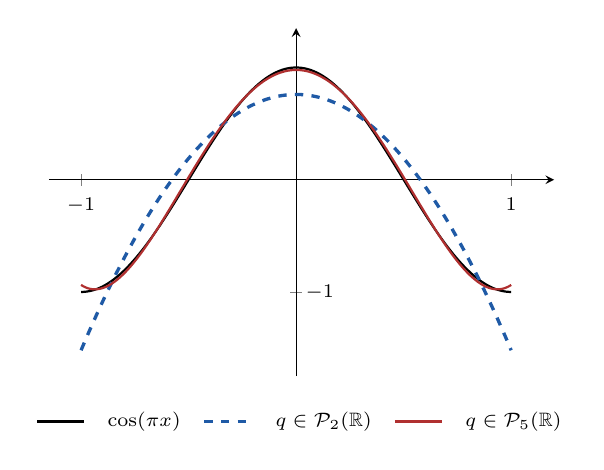
\begin{tikzpicture}
\begin{axis}[width=8cm,height=6cm,axis lines=middle,axis line style={-stealth,thin},
  xmin=-1.15,xmax=1.2,ymin=-1.75,ymax=1.35,xtick={-1,1},ytick={-1},
  ticklabel style={font=\scriptsize},x tick label style={anchor=north,yshift=-1pt},y tick label style={anchor=west,xshift=2pt},
  legend style={font=\scriptsize,at={(0.5,-0.07)},anchor=north,legend columns=3,column sep=6pt,draw=none,fill=white,fill opacity=0.85,text opacity=1,cells={anchor=west}},
  samples=200,domain=-1:1]
\addplot[black,thick] {cos(deg(pi*x))}; \addlegendentry{$\cos(\pi x)$}
\addplot[figB,very thick,dashed] {15/(2*pi^2)*(1-3*x^2)}; \addlegendentry{$q\in\mathcal P_2(\mathbb R)$}
\addplot[figR,thick] {105/(8*pi^4)*((27-2*pi^2)+(24*pi^2-270)*x^2+(315-30*pi^2)*x^4)}; \addlegendentry{$q\in\mathcal P_5(\mathbb R)$}
\end{axis}\end{tikzpicture}\end{document}
